\input format.tex

\usepackage{graphicx}
\graphicspath{{cores/}}
\usepackage{setspace}

\newcolumntype{K}[1]{>{\centering\arraybackslash}p{#1}}

\begin{document}

\vspace*{6mm}

\noindent\fcolorbox{topcolor}{topcolor}{
\parbox[c][1cm]{\textwidth}{
\begin{center}
\fontsize{18pt}{\baselineskip}\selectfont\color{white}{\bf {肠道益生菌检测结果}}
\end{center}
}
}


%% 各章节
\setlength{\arrayrulewidth}{1pt}
\fontsize{8pt}{11pt}\selectfont
\color{black70}

\vspace*{3mm}

\fontsize{11pt}{13pt}\selectfont
\noindent\begin{tabular}{p{4.8cm}p{5.2cm}}
\parbox[c]{\hsize}{\vskip7pt 姓名:Jessica \vskip7pt} & 年龄:28 \\
\parbox[c]{\hsize}{\vskip7pt 样本编码:tptest002 \vskip7pt} & 送检机构:湘雅附三体检中心 \\
\end{tabular}

\begin{LRaside2}{\bf 您本次肠道益生菌总评分如下}
\begin{center}
\setlength{\unitlength}{1cm}
\begin{picture}(20,2.6)(0,-0.8)
\put(1.92105263157895,0.55){
\includegraphics[scale=1]{straw_l2.pdf}}
\put(0.5,-0.2){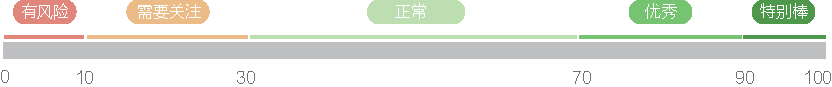
\includegraphics[scale=1]{baohulibar03.pdf}}
\end{picture}
\indent\fontsize{9pt}{11pt}\selectfont\bf {综合您本次肠道益生菌检测,您本次益生菌检测总评分为
{\fontsize{13pt}{14pt}\selectfont\color{level2} 11分},需要关注
}

\includegraphics[scale=1]{underline.pdf}
\end{center}
{\par\fontsize{9pt}{11pt}\selectfont\bf {您需要通过饮食、补充微生态制剂、运动等方式来改善肠道菌群情况。肠道益生菌评分越高,说明您的肠道越健康;反之,肠
道益生菌评分越低,则说明您的肠道微生态环境越值得关注。}}
\end{LRaside2}

\vspace*{-2mm}
\hspace*{12.5cm}
\raisebox{-0.4ex}{\includegraphics{drop_l2.pdf}}
\fontsize{9pt}{11pt}\selectfont {本次检测结果}

\vspace*{5mm}

\noindent\fontsize{11pt}{12pt}\selectfont {\bf 综合健康建议}
\noindent
\fontsize{8pt}{11pt}\selectfont
\setlength{\arrayrulewidth}{.5pt}
\begin{center}
\begin{tabular}{K{1.3cm}K{13.6cm}}
\hline

\parbox[c][2.5cm]{.95\hsize}{
\noindent

\includegraphics[scale=1.0]{diet.pdf}
}
 &
%\hspace*{1mm}
\parbox{\hsize}{
\vspace*{0.5mm}
\begin{spacing}{1.5}
{
\includegraphics[scale=1.0]{xiaoyuandian.pdf}\fontsize{8.5pt}{10pt}\selectfont \ 建议您在日常饮食中选择补充糙米、南瓜、海军豆等食物或者相关的加工提取食品,为肠道菌群提供更多营养,促进有益共生菌的生长,增加肠道菌群的丰富度及多样性。 \\}
{
\includegraphics[scale=1.0]{xiaoyuandian.pdf}\fontsize{8.5pt}{10pt}\selectfont \ 控制油炸类、西式快餐、含糖饮料等高脂高糖高热量食物。忌暴饮暴食。减少外出就餐。戒烟限酒。}
\end{spacing}
} \\
\hline

\parbox[c][2.5cm]{.95\hsize}{
\noindent

\includegraphics[scale=1.0]{probiotics.pdf}
}
 &
%\hspace*{1mm}
\parbox{\hsize}{
\vspace*{0.5mm}
\begin{spacing}{1.5}
{
\includegraphics[scale=1.0]{xiaoyuandian.pdf}\fontsize{8.5pt}{10pt}\selectfont \ 建议您选择补充含BB-12的酸奶、含保加利亚乳杆菌的酸奶、含干酪乳杆菌的活菌饮料等益生菌产品,以增加您肠道内益生菌的含量,并能抑制有害菌的异常增殖,调节肠道菌群平衡。 \\}
{
\includegraphics[scale=1.0]{xiaoyuandian.pdf}\fontsize{8.5pt}{10pt}\selectfont \ 选酸奶有窍门,2型糖尿病、动脉粥样硬化、胆囊炎、胰腺炎等患者,宜选用无糖酸奶。}
\end{spacing}
} \\
\hline

\parbox[c][2.5cm]{.95\hsize}{
\noindent

\includegraphics[scale=1.0]{prebiotics.pdf}
}
 &
%\hspace*{1mm}
\parbox{\hsize}{
\vspace*{0.5mm}
\begin{spacing}{1.5}
{
\includegraphics[scale=1.0]{xiaoyuandian.pdf}\fontsize{8.5pt}{10pt}\selectfont \ 建议您选择补充低聚果糖、菊粉、富含多酚的蔓越莓提取物等益生元,能帮助柔嫩梭菌属、阿克曼氏菌属、双歧杆菌属、乳酸杆菌属在肠道内增殖,增加有益物质的产生,有利于增强肠道屏障功能,促进肠道健康。 \\}
{
\includegraphics[scale=1.0]{xiaoyuandian.pdf}\fontsize{8.5pt}{10pt}\selectfont \ 如患炎症性肠病、腹泻,避免菊粉和膳食纤维制剂的摄入。}
\end{spacing}
} \\
\hline

\end{tabular}
\end{center}


\end{document}

